

\tikzset{every picture/.style={line width=0.75pt}} %set default line width to 0.75pt        

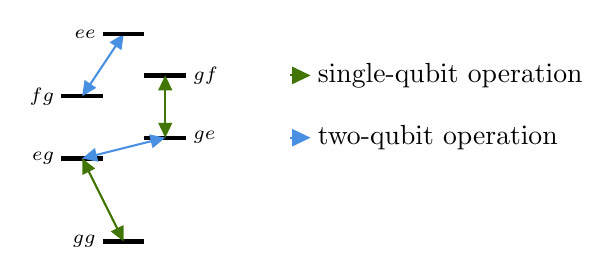
\begin{tikzpicture}[x=0.75pt,y=0.75pt,yscale=-1,xscale=1]
%uncomment if require: \path (0,300); %set diagram left start at 0, and has height of 300

%Straight Lines [id:da9559663622579351] 
\draw [line width=1.5]    (100,100) -- (120,100) ;
%Straight Lines [id:da38130444644691297] 
\draw [line width=1.5]    (140,90) -- (160,90) ;
%Straight Lines [id:da2359488638530448] 
\draw [line width=1.5]    (100,130) -- (120,130) ;
%Straight Lines [id:da3841009239924672] 
\draw [line width=1.5]    (120,170) -- (140,170) ;
%Straight Lines [id:da5788606590900368] 
\draw [line width=1.5]    (140,120) -- (160,120) ;
%Straight Lines [id:da9477773949836692] 
\draw [color={rgb, 255:red, 65; green, 117; blue, 5 }  ,draw opacity=1 ]   (111.34,132.68) -- (128.66,167.32) ;
\draw [shift={(130,170)}, rotate = 243.43] [fill={rgb, 255:red, 65; green, 117; blue, 5 }  ,fill opacity=1 ][line width=0.08]  [draw opacity=0] (7.14,-3.43) -- (0,0) -- (7.14,3.43) -- cycle    ;
\draw [shift={(110,130)}, rotate = 63.43] [fill={rgb, 255:red, 65; green, 117; blue, 5 }  ,fill opacity=1 ][line width=0.08]  [draw opacity=0] (7.14,-3.43) -- (0,0) -- (7.14,3.43) -- cycle    ;
%Straight Lines [id:da6539701699881647] 
\draw [color={rgb, 255:red, 74; green, 144; blue, 226 }  ,draw opacity=1 ]   (128.34,72.5) -- (111.66,97.5) ;
\draw [shift={(110,100)}, rotate = 303.69] [fill={rgb, 255:red, 74; green, 144; blue, 226 }  ,fill opacity=1 ][line width=0.08]  [draw opacity=0] (7.14,-3.43) -- (0,0) -- (7.14,3.43) -- cycle    ;
\draw [shift={(130,70)}, rotate = 123.69] [fill={rgb, 255:red, 74; green, 144; blue, 226 }  ,fill opacity=1 ][line width=0.08]  [draw opacity=0] (7.14,-3.43) -- (0,0) -- (7.14,3.43) -- cycle    ;
%Straight Lines [id:da6430626577491835] 
\draw [color={rgb, 255:red, 65; green, 117; blue, 5 }  ,draw opacity=1 ]   (210,90) -- (217,90) ;
\draw [shift={(220,90)}, rotate = 180] [fill={rgb, 255:red, 65; green, 117; blue, 5 }  ,fill opacity=1 ][line width=0.08]  [draw opacity=0] (8.93,-4.29) -- (0,0) -- (8.93,4.29) -- cycle    ;
%Straight Lines [id:da593444231277527] 
\draw [color={rgb, 255:red, 74; green, 144; blue, 226 }  ,draw opacity=1 ]   (210,120) -- (217,120) ;
\draw [shift={(220,120)}, rotate = 180] [fill={rgb, 255:red, 74; green, 144; blue, 226 }  ,fill opacity=1 ][line width=0.08]  [draw opacity=0] (8.93,-4.29) -- (0,0) -- (8.93,4.29) -- cycle    ;
%Straight Lines [id:da04551771823475548] 
\draw [line width=1.5]    (120,70) -- (140,70) ;
%Straight Lines [id:da8060801042251682] 
\draw [color={rgb, 255:red, 65; green, 117; blue, 5 }  ,draw opacity=1 ]   (150,93) -- (150,117) ;
\draw [shift={(150,120)}, rotate = 270] [fill={rgb, 255:red, 65; green, 117; blue, 5 }  ,fill opacity=1 ][line width=0.08]  [draw opacity=0] (7.14,-3.43) -- (0,0) -- (7.14,3.43) -- cycle    ;
\draw [shift={(150,90)}, rotate = 90] [fill={rgb, 255:red, 65; green, 117; blue, 5 }  ,fill opacity=1 ][line width=0.08]  [draw opacity=0] (7.14,-3.43) -- (0,0) -- (7.14,3.43) -- cycle    ;
%Straight Lines [id:da40683969551339827] 
\draw [color={rgb, 255:red, 74; green, 144; blue, 226 }  ,draw opacity=1 ]   (112.91,129.27) -- (147.09,120.73) ;
\draw [shift={(150,120)}, rotate = 165.96] [fill={rgb, 255:red, 74; green, 144; blue, 226 }  ,fill opacity=1 ][line width=0.08]  [draw opacity=0] (7.14,-3.43) -- (0,0) -- (7.14,3.43) -- cycle    ;
\draw [shift={(110,130)}, rotate = 345.96] [fill={rgb, 255:red, 74; green, 144; blue, 226 }  ,fill opacity=1 ][line width=0.08]  [draw opacity=0] (7.14,-3.43) -- (0,0) -- (7.14,3.43) -- cycle    ;

% Text Node
\draw (98,100) node [anchor=east] [inner sep=0.75pt]  [font=\scriptsize]  {$fg$};
% Text Node
\draw (98,130) node [anchor=east] [inner sep=0.75pt]  [font=\scriptsize]  {$eg$};
% Text Node
\draw (118,170) node [anchor=east] [inner sep=0.75pt]  [font=\scriptsize]  {$gg$};
% Text Node
\draw (162,90) node [anchor=west] [inner sep=0.75pt]  [font=\scriptsize]  {$gf$};
% Text Node
\draw (162,120) node [anchor=west] [inner sep=0.75pt]  [font=\scriptsize]  {$ge$};
% Text Node
\draw (222,90) node [anchor=west] [inner sep=0.75pt]   [align=left] {single-qubit operation};
% Text Node
\draw (222,120) node [anchor=west] [inner sep=0.75pt]   [align=left] {two-qubit operation};
% Text Node
\draw (118,70) node [anchor=east] [inner sep=0.75pt]  [font=\scriptsize]  {$ee$};


\end{tikzpicture}